\documentclass[acmsmall]{acmart}

\usepackage{booktabs} % For formal tables


% \usepackage[ruled]{algorithm2e} % For algorithms

\usepackage{cleveref}
\usepackage{epsfig}
\usepackage{float}
\usepackage{amsmath,amssymb,amsfonts}
\usepackage{algorithm}
\usepackage[noend]{algpseudocode}
\usepackage{bigstrut,multirow}
\usepackage{threeparttable}
\usepackage{subfigure}

% \renewcommand{\algorithmcfname}{ALGORITHM}
% \SetAlFnt{\small}
% \SetAlCapFnt{\small}
% \SetAlCapNameFnt{\small}
% \SetAlCapHSkip{0pt}
% \IncMargin{-\parindent}

% Metadata Information
\acmJournal{TRETS}
\acmVolume{9}
\acmNumber{4}
\acmArticle{11}
\acmYear{2017}
\acmMonth{12}
\acmArticleSeq{11}

%\acmBadgeR[http://ctuning.org/ae/ppopp2016.html]{ae-logo}
%\acmBadgeL[http://ctuning.org/ae/ppopp2016.html]{ae-logo}


% Copyright
%\setcopyright{acmcopyright}
%\setcopyright{acmlicensed}
%\setcopyright{rightsretained}
%\setcopyright{usgov}
\setcopyright{usgovmixed}
%\setcopyright{cagov}
%\setcopyright{cagovmixed}

% DOI
\acmDOI{0000001.0000001}

% Paper history
% \received{February 2007}
% \received{March 2009}
% \received[accepted]{June 2009}


% Document starts
\begin{document}
% Title portion
\title{[DL] A Survey of FPGA Based Neural Network Accelerator} 
% \titlenote{We can add a note to the title}

\author{Kaiyuan Guo, Shulin Zeng, Jincheng Yu, Yu Wang {\scshape and} Huazhong Yang}
% \authornote{This is the corresponding author}
% \orcid{1234-5678-9012-3456}
\affiliation{%
  \institution{Tsinghua University}
  \streetaddress{Tsinghua University}
  \city{Beijing}
  \state{Beijing}
  \postcode{100084}
  \country{China}}
\email{gky15@mails.tsinghua.edu.cn, yu-wang@mail.tsinghua.edu.cn}

% \author{Yiming Hu}
% \authornote{This is the corresponding author}
% \orcid{1234-5678-9012-3456}
% \affiliation{%
%   \institution{Tsinghua University}
%   \streetaddress{Tsinghua University}
%   \city{Beijing}
%   \state{Beijing}
%   \postcode{100084}
%   \country{China}}
% \email{hym16@mails.tsinghua.edu.cn}


%
% The code below should be generated by the tool at
% http://dl.acm.org/ccs.cfm
% Please copy and paste the code instead of the example below. 
%

\begin{abstract}

Recent researches on neural network have shown significant advantage in machine learning over traditional algorithms based on handcrafted features and models. Neural network is now widely adopted in regions like image, speech and video recognition. But the high computation and storage complexity of neural network inference poses great difficulty on its application. CPU platforms are hard to offer enough computation capacity. GPU platforms are the first choice for neural network process because of its high computation capacity and easy to use development frameworks. 

On the other hand, FPGA-based neural network inference accelerator is becoming a research topic. With specifically designed hardware, FPGA is the next possible solution to surpass GPU in speed and energy efficiency. Various FPGA-based accelerator designs have been proposed with software and hardware optimization techniques to achieve high speed and energy efficiency. In this paper, we give an overview of previous work on neural network inference accelerators based on FPGA and summarize the main techniques used. An investigation from software to hardware, from circuit level to system level is carried out to complete analysis of FPGA-based neural network inference accelerator design and serves as a guide to future work. 

\end{abstract}

\begin{CCSXML}
  <ccs2012>
  <concept>
  <concept_id>10010520.10010553.10010562.10010563</concept_id>
  <concept_desc>Computer systems organization~Embedded hardware</concept_desc>
  <concept_significance>500</concept_significance>
  </concept>
  <concept>
  <concept_id>10010520.10010570.10010574</concept_id>
  <concept_desc>Computer systems organization~Real-time system architecture</concept_desc>
  <concept_significance>300</concept_significance>
  </concept>
  </ccs2012>
  \end{CCSXML}
  
  \ccsdesc[500]{Computer systems organization~Embedded hardware}
  \ccsdesc[300]{Computer systems organization~Real-time system architecture}

\end{CCSXML}
%
% End generated code
%


\keywords{FPGA, Neural Network}

% DO NOT use this command unless you want to change
% the default behavior
% \authorsaddresses{Authors' addresses: G.~Zhou, Computer Science
%   Department, College of William and Mary, 104 Jameson Rd,
%   Williamsburg, PA 23185, US, \path{gzhou@wm.edu}; V.~B\'eranger,
%   Inria Paris-Rocquencourt, Rocquencourt, France; A.~Patel, Rajiv
%   Gandhi University, Rono-Hills, Doimukh, Arunachal Pradesh, India;
%   H.~Chan, Tsinghua University, 30 Shuangqing Rd, Haidian Qu, Beijing
%   Shi, China; T.~Yan, Eaton Innovation Center, Prague, Czech Republic;
%   T.~He, C.~Huang, J.~A.~Stankovic University of Virginia, School of
%   Engineering Charlottesville, VA 22903, USA; T. F. Abdelzaher,
%   (Current address) NASA Ames Research Center, Moffett Field,
%   California 94035.}

\maketitle

% The default list of authors is too long for headers.
\renewcommand{\shortauthors}{K. Guo et al.}

\section{Introduction}\label{sec:introduction}

Recent research on Neural Network (NN) is showing great improvement over traditional algorithms in computer vision. Various network models, like convolutional neural network (CNN), recurrent neural network (RNN), have been proposed for image, video, and speech process. CNN~\cite{krizhevsky2012imagenet} improves the top-5 image classification accuracy on ImageNet~\cite{ILSVRC15} dataset from 73.8\% to 84.7\% and further helps improve object detection~\cite{girshick2014rich} with its outstanding ability in feature extraction. RNN~\cite{hannun2014deep} achieves state-of-the-art word error rate on speech recognition. In general, NN features a high fitting ability to a wide range of pattern recognition problems. This makes NN a promising candidate to many artificial intelligence applications.

But the computation and storage complexity of NN models are high. The research on NN is also increasing the size of NN models. The largest neural network model for an $224\times224$ image classification requires upto 39 billion floating point operations (FLOP) and more than 500MB model parameters~\cite{simonyan2014very}. As the computation complexity is propotional to the input image size, processing images with higher resolutions may need more than 100 billion operations.

Traditional hardware platforms are not suitable for neural network process. A common CPU can perform 10-100G FLOP per second, and the power efficieny is usually below 1GOPs/W. So CPUs neither meet the high performance requirements in cloud applications nor the low power requiremetns in mobile applications. In contrast, GPUs offer upto 10TOP/s peak performance and is a good choice for high performance neural network applications. Development frameworks like Caffe~\cite{jia2014caffe} and Tensorflow~\cite{abadi2016tensorflow} also offers easy-to-use interfaces which makes GPU the first choice of neural network acceleration. But GPUs are power consuming and thus not suitable for mobile applications.

On the other hand, FPGA is becoming a candidate to implement energy efficient neural network accelerator. With a specific hardware design, FPGAs are able to implement high parallelism and make use of the properties of neural network computation to remove unecessary logic. Therefore FPGAs are possible to achieve higher energy efficieny compared with CPU and GPU. 

But FPGA based accelerator designs are still faced with two problems:
\begin{itemize}
    \item Current FPGAs usually support working frequency at 100-300MHz, which is much less than CPU and GPU. The FPGA's logic overhead for reconfigurability also reduces the overall system performance. Straight forward design on FPGA is hard to achieve high performance and high energy efficiency.
    \item Implementation of neural networks on FPGAs is much harder than that on CPUs or GPUs. Development framework like Caffe and Tensorflow for CPU and GPU is needed for FPGA.
\end{itemize}
 
Many researches on the above two problems have been carried out for energy efficient and flexible FPGA based neural network accelerator. In this paper, we summarize the techniques proposed in these work. Specifically, we will introduce the techiques from the following aspects:
\begin{itemize}
    \item We investigate current techniques for high performance and energy efficient neural network accelerator designs. Techniques in both software level and hardware level are evaluated.
    \item We investigate state-of-the-art automatic design methods of FPGA based neural network accelerators. 
\end{itemize}

The rest part of this paper is organized as follows:

\section{Preliminary}\label{sec:preliminary}

\rev{Before discussing the system design for neural network acceleration, we first introduce the basic concepts of neural networks and the basic components of an FPGA-based accelerator design.}

\subsection{Neural Network}

\begin{figure}[ht]
    \centering
    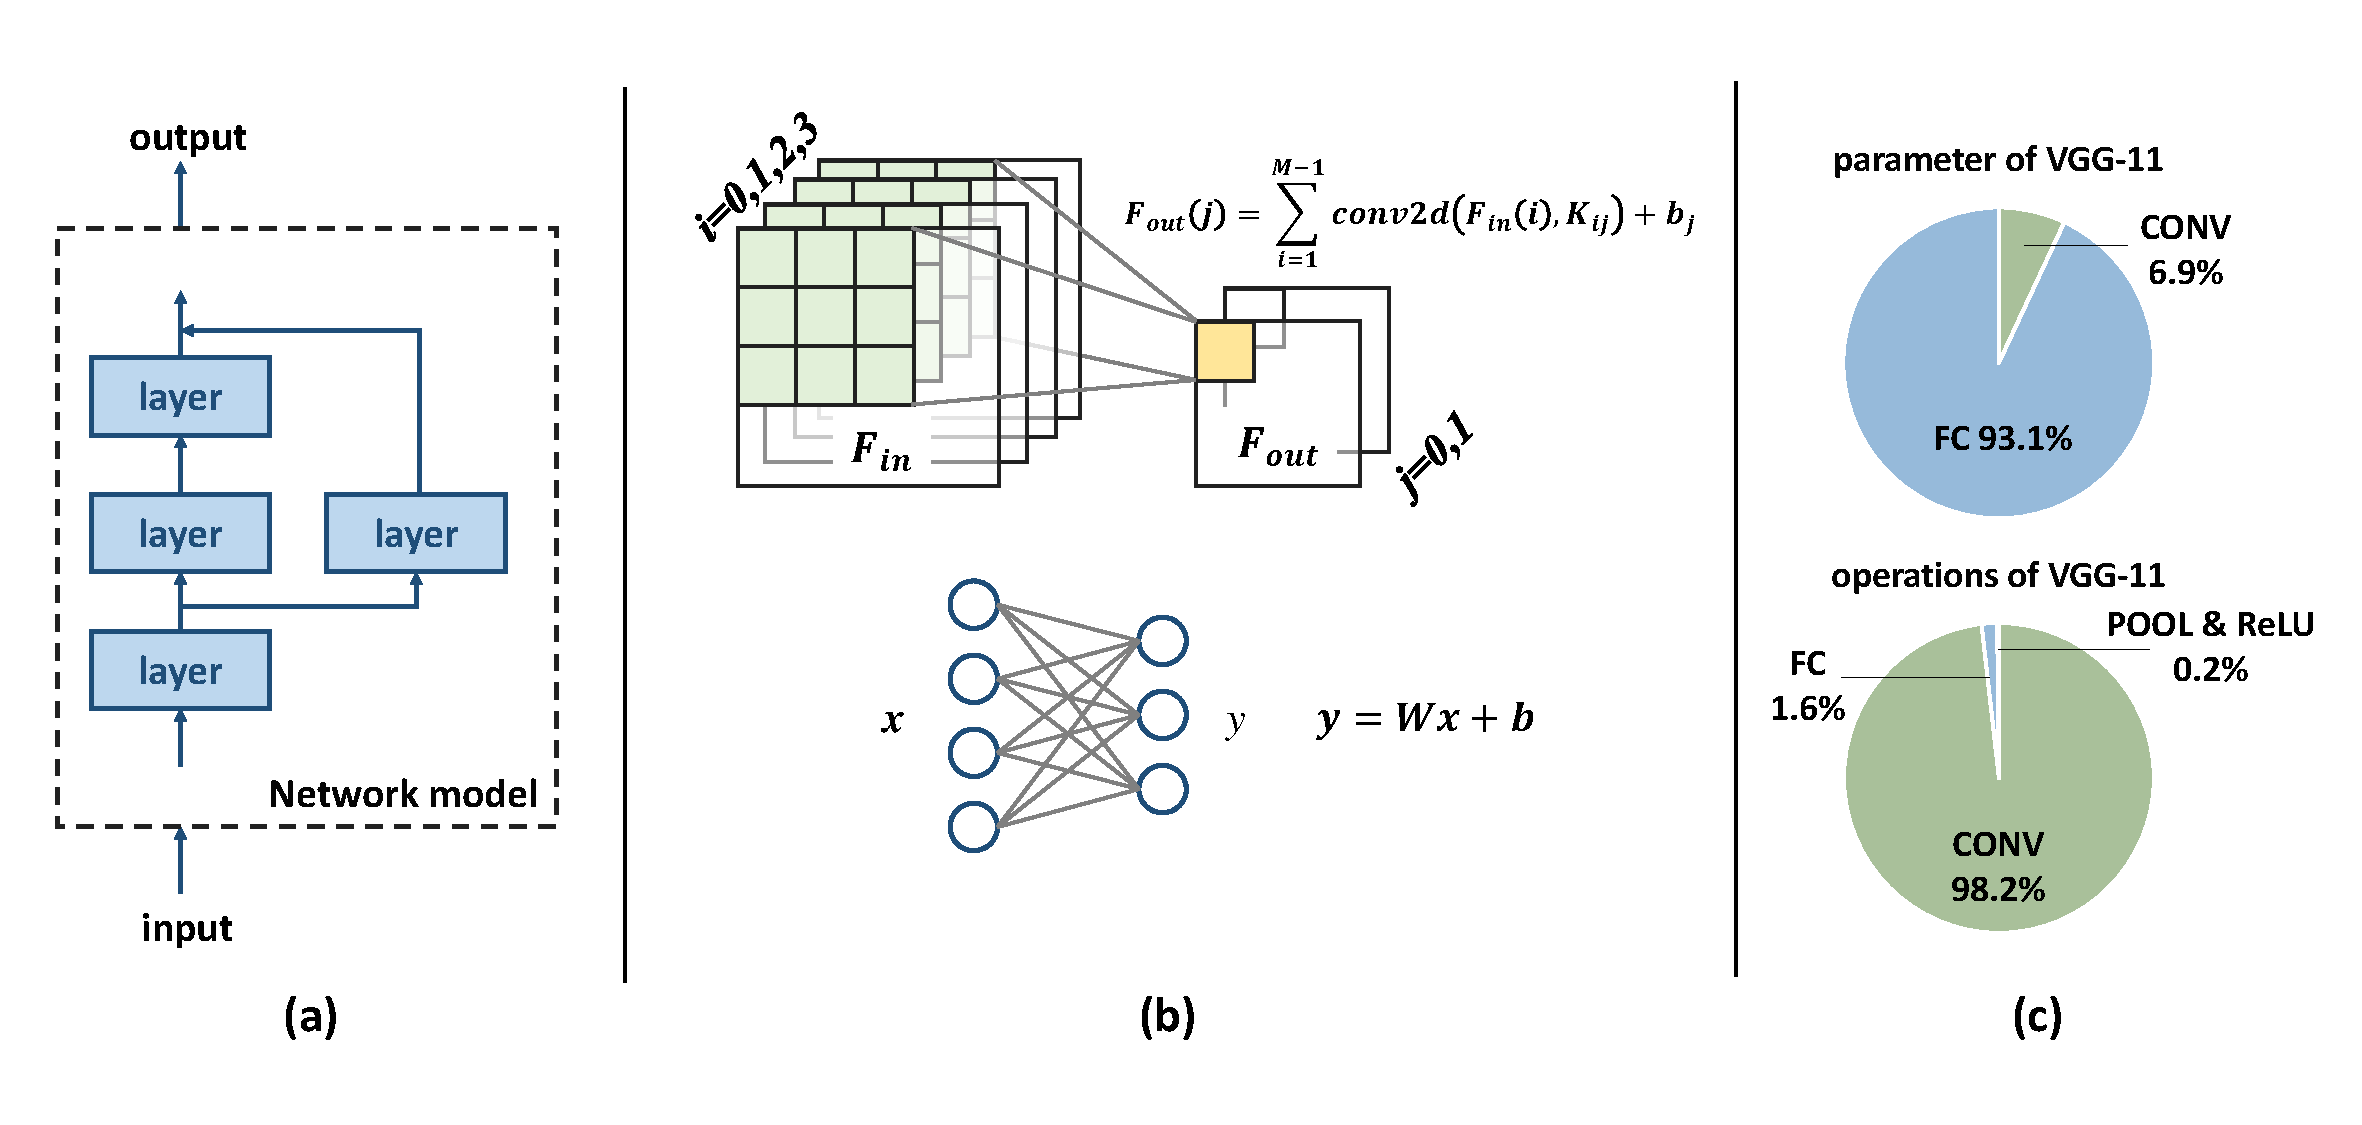
\includegraphics[width=1.0\columnwidth]{fig/cnn_preliminary.pdf}
    \caption{\rev{(a) Computation graph of a neural network model. (b) CONV and FC layers in NN model. (c) CONV and FC layers dominates the computation and parameter of a NN model.}}
    \label{fig:cnn_preliminary}
\end{figure}

\rev{In this section, we introduce the basic functions in a neural network. A neural network model can be described as a directed graph shown in Figure~\ref{fig:cnn_preliminary}(a). Each vertex of the graph denotes a layer which conducts operations on data from a previous layer or input and generates results to the next layer or output.

Convolution (CONV) layers and fully connected (FC) layers are two common types of layers in NN models. The functions of these two layers are shown in Figure~\ref{fig:cnn_preliminary}(b). CONV layers conduct 2D convolutions on a set of input feature maps $F_{in}$ and add the results to get output feature maps $F_{out}$. FC layers receives a feature vector as input and conduct matrix-vector multiplications.

Besides CONV and FC layers, NN layers also have pooling, ReLU~\cite{krizhevsky2012imagenet}, concat~\cite{szegedy2015going}, element-wise~\cite{he2016deep} and other types of layers. But these layers contributes little to the computation and storage requirement of a neural network model. Figure~\ref{fig:cnn_preliminary}(c) shows the distribution of parameter and operations in the VGG-11 model~\cite{simonyan2014very}. CONV and FC layers together contributes more than 99\% of the network's parameters and operations. So most of the neural network acceleration systems focus on these two types of layers.
}

\subsection{FPGA-based Accelerator}

\rev{In recent years, FPGA is becoming a promising solution for accelerating certain algorithms. Compared with CPU, GPU, and DSP platforms, for which the software and hardware are designed independently, FPGA enables the developers to implement only the necessary logic in hardware according to the target algorithm. By eliminating the redundancy in general hardware platforms, FPGAs are able to achieve higher efficiency. Application specific integrated circuits (ASICs) based solutions achieves even higher efficiency, but requires much longer development cycle and higher cost. 

\begin{figure}[ht]
    \centering
    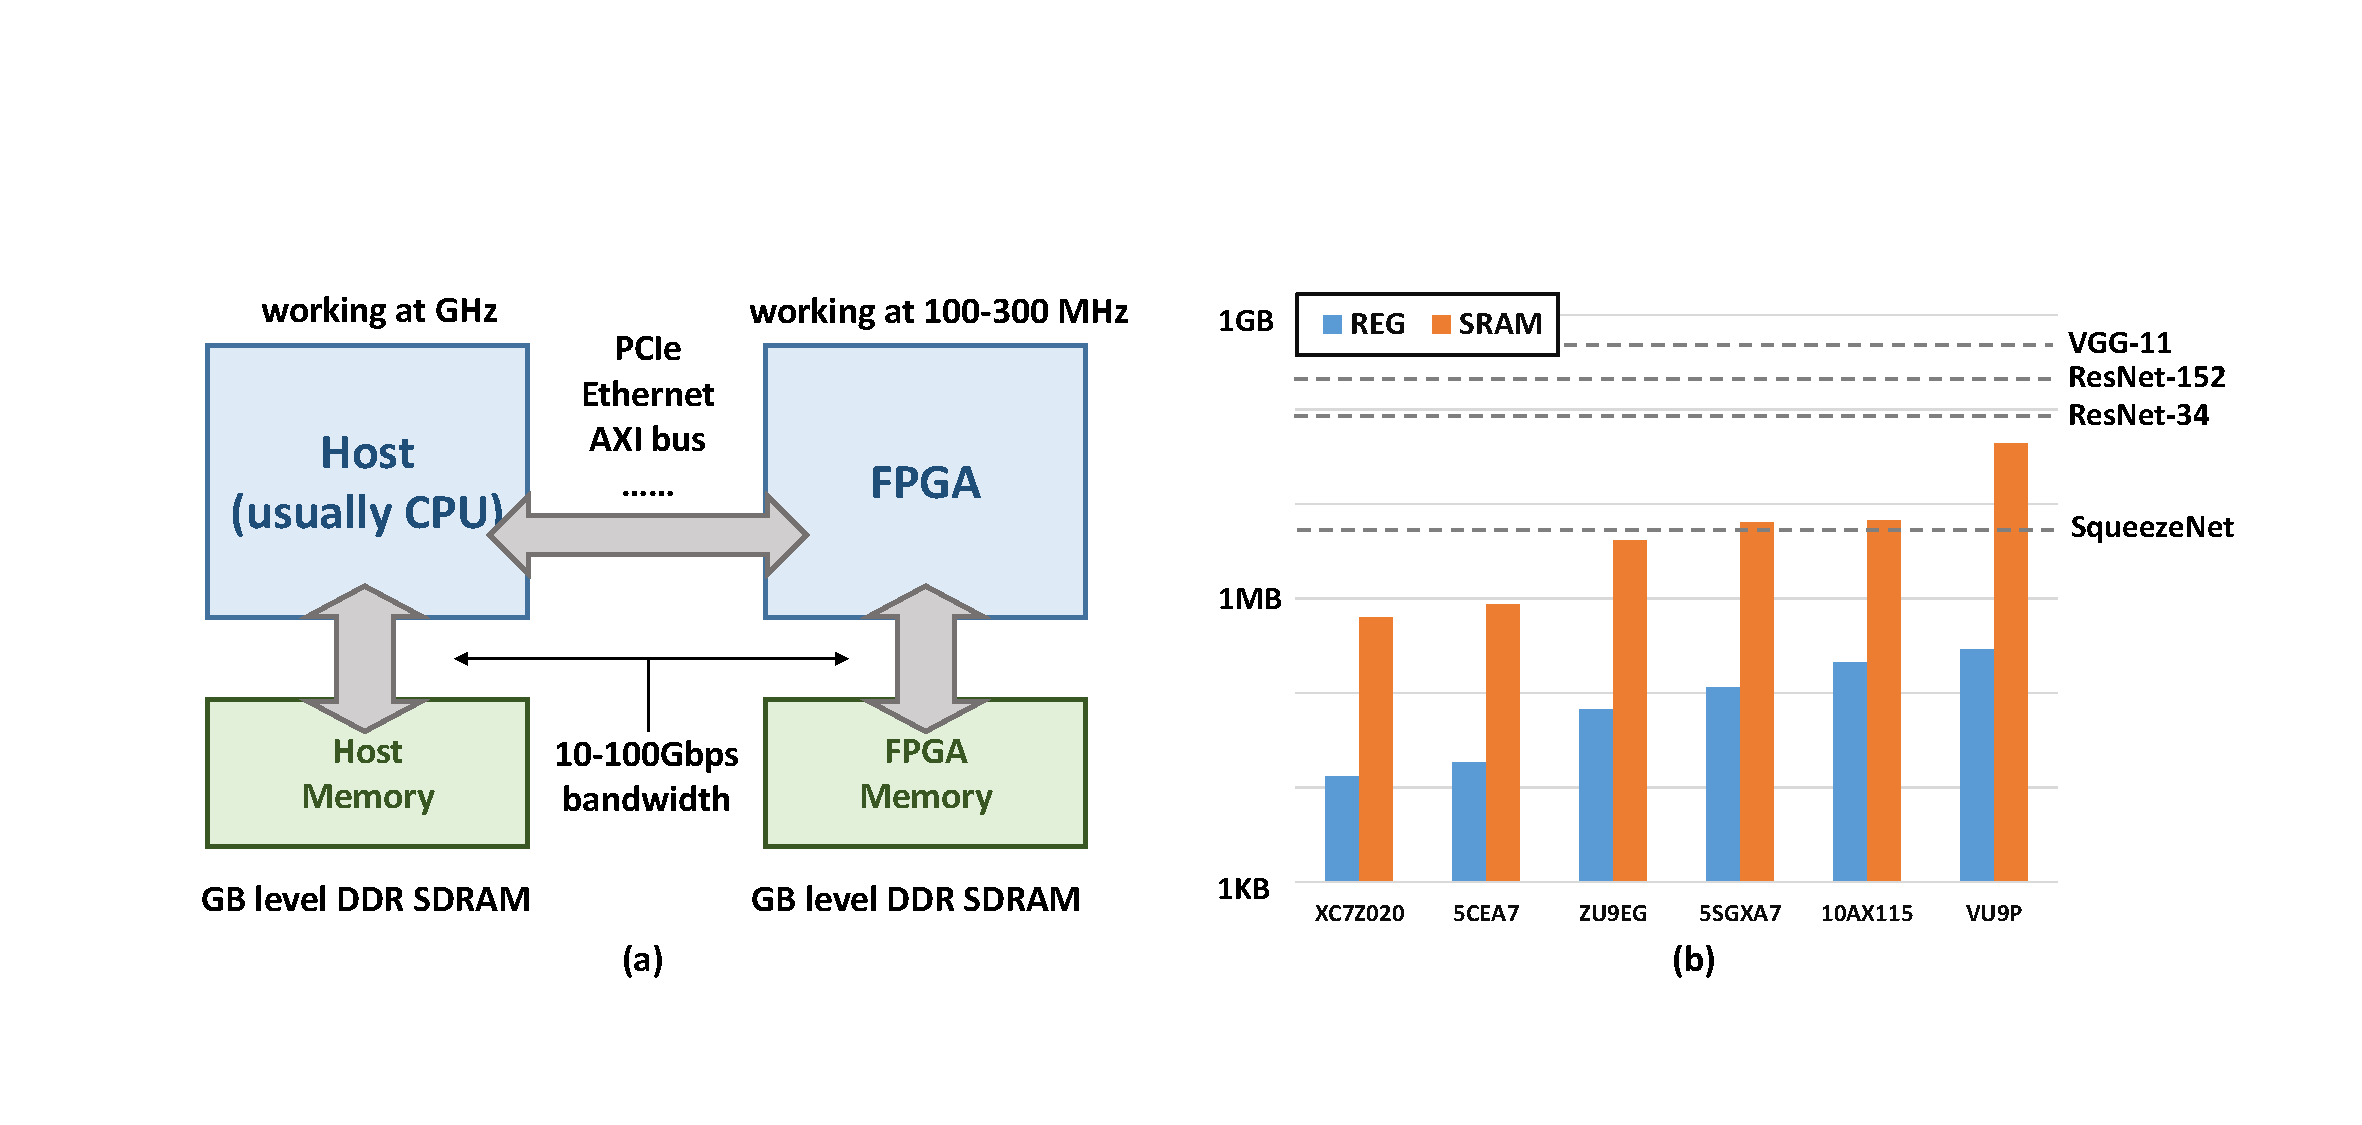
\includegraphics[width=0.8\columnwidth]{fig/fpga_preliminary.pdf}
    \caption{\rev{(a) A typical structure of an FPGA based NN accelerator. (b) Comparison between NN model size and the storage on different FPGA chips.}}
    \label{fig:fpga_preliminary}
\end{figure}

For FPGA-based neural network accelerator, a typical architecture of the system is shown in Figure~\ref{fig:fpga_preliminary}(a). The system usually consists of a CPU host and an FPGA part. A pure FPGA chip usually works with a host PC/server through PCIe connections. SoC platforms (like the Xilinx Zynq Series) and Intel HARPv2~\cite{gupta2016accelerating} platform integrates the host and the FPGA in the same chip or package. Both the host and the FPGA can work with their own external memory and access each others' memory through the connection. Most of the designs implements NN accelerator on the FPGA part and controls the 
acceleartor with the software on the host.

Typical FPGA chips implement large on-chip storage units like registers and SRAMs, but still too small compared with NN models as shown in Figure~\ref{fig:fpga_preliminary}(b). Common models implement 100-1000MB parameters while the largest available FPGA chip implements <50MB on-chip SRAM. This requires that external memory like DDR SDRAM is needed. The bandwidth and power consumption of DDR limits the system performance.

Compared with storage, the computation capacity of FPGA is relatively higher. Common FPGAs implements hundreds to thousands of DSP units, each of which can compute $18\times 27$ or $18\times 19$, achieving upto 10TFLOP/s (floating point operations per second) on the largest FPGAs. But for low-end FPGAs like Xilinx XC7Z020, this number is reduced to 20GFLOP/s, which is hard to support real-time video processing for applications on mobile platforms. 

Even faced with the above challenges, researchers have proposed a series of optimization methods from algorithm to architecture to design high performance NN accelerators on FPGA, which will be discussed in the following sections of this paper.}

\bibliographystyle{ACM-Reference-Format}
\bibliography{ref}

\end{document}
